\paragraph{Desarrollo técnico}
El objetivo de este circuito estaba pensado para dar una aplicaci\'on a la señal digital recibida por el receptor. El circuito consistía en una máquina de estados cuya salida tenía una aplicación concreta. En este caso, por cada señal recibida, poner en alto una de sus salidas, manteniendo el estado de las anteriores hasta completar el ciclo, donde todas volverían a estado bajo. 
El esquemático del circuito digital de la máquina de estados se muestra en la figura \ref{fig:crono_logisim}.
Además, se añade en la figura \ref{fig:crono_general}, la integración del receptor superheterodino FM anterior, junto al circuito digital montados en una placa de entrenamiento.

\begin{figure}[h!]
    \centering
    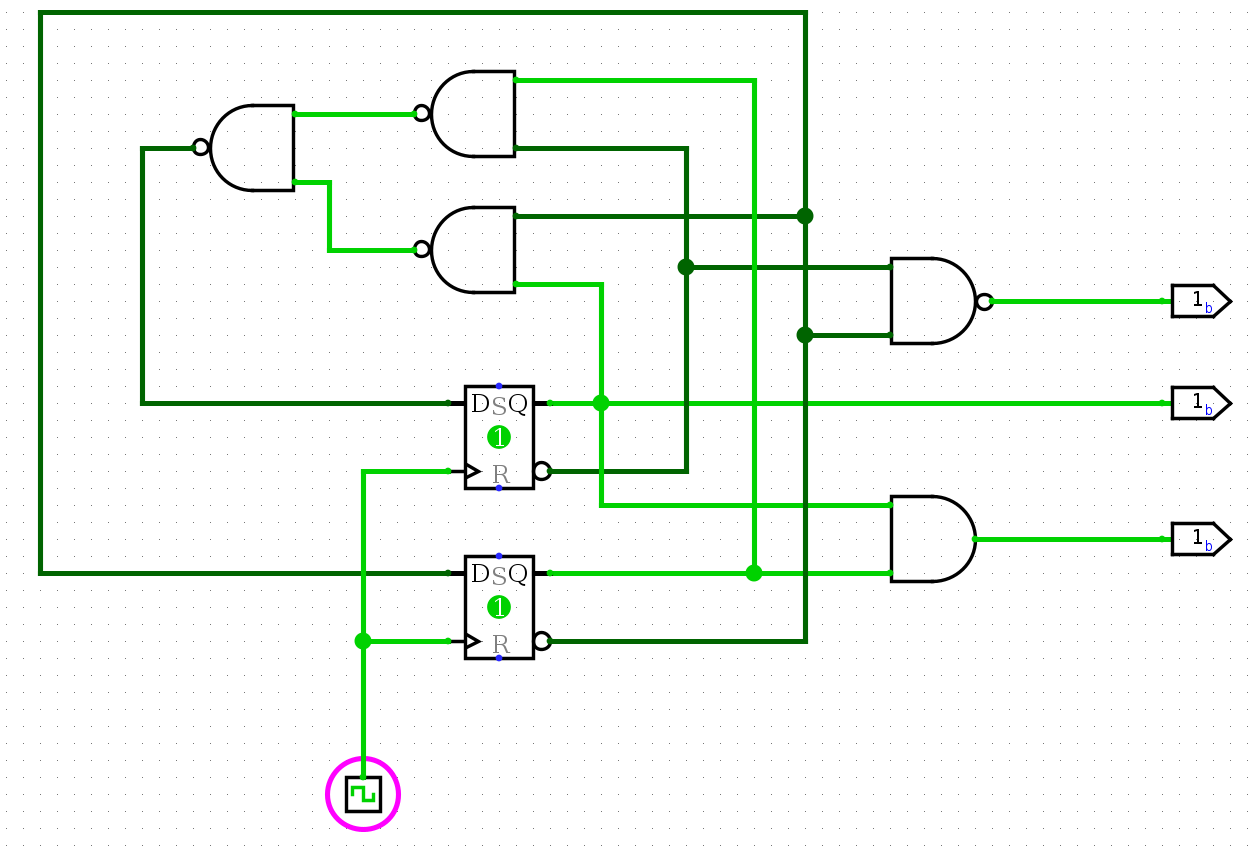
\includegraphics[scale=1, width=.6\textwidth]{crono_logisim}
    \caption{Esquemático de la m\'aquina estados}
    \label{fig:crono_logisim}
\end{figure}

\begin{figure}[h!]
    \centering
    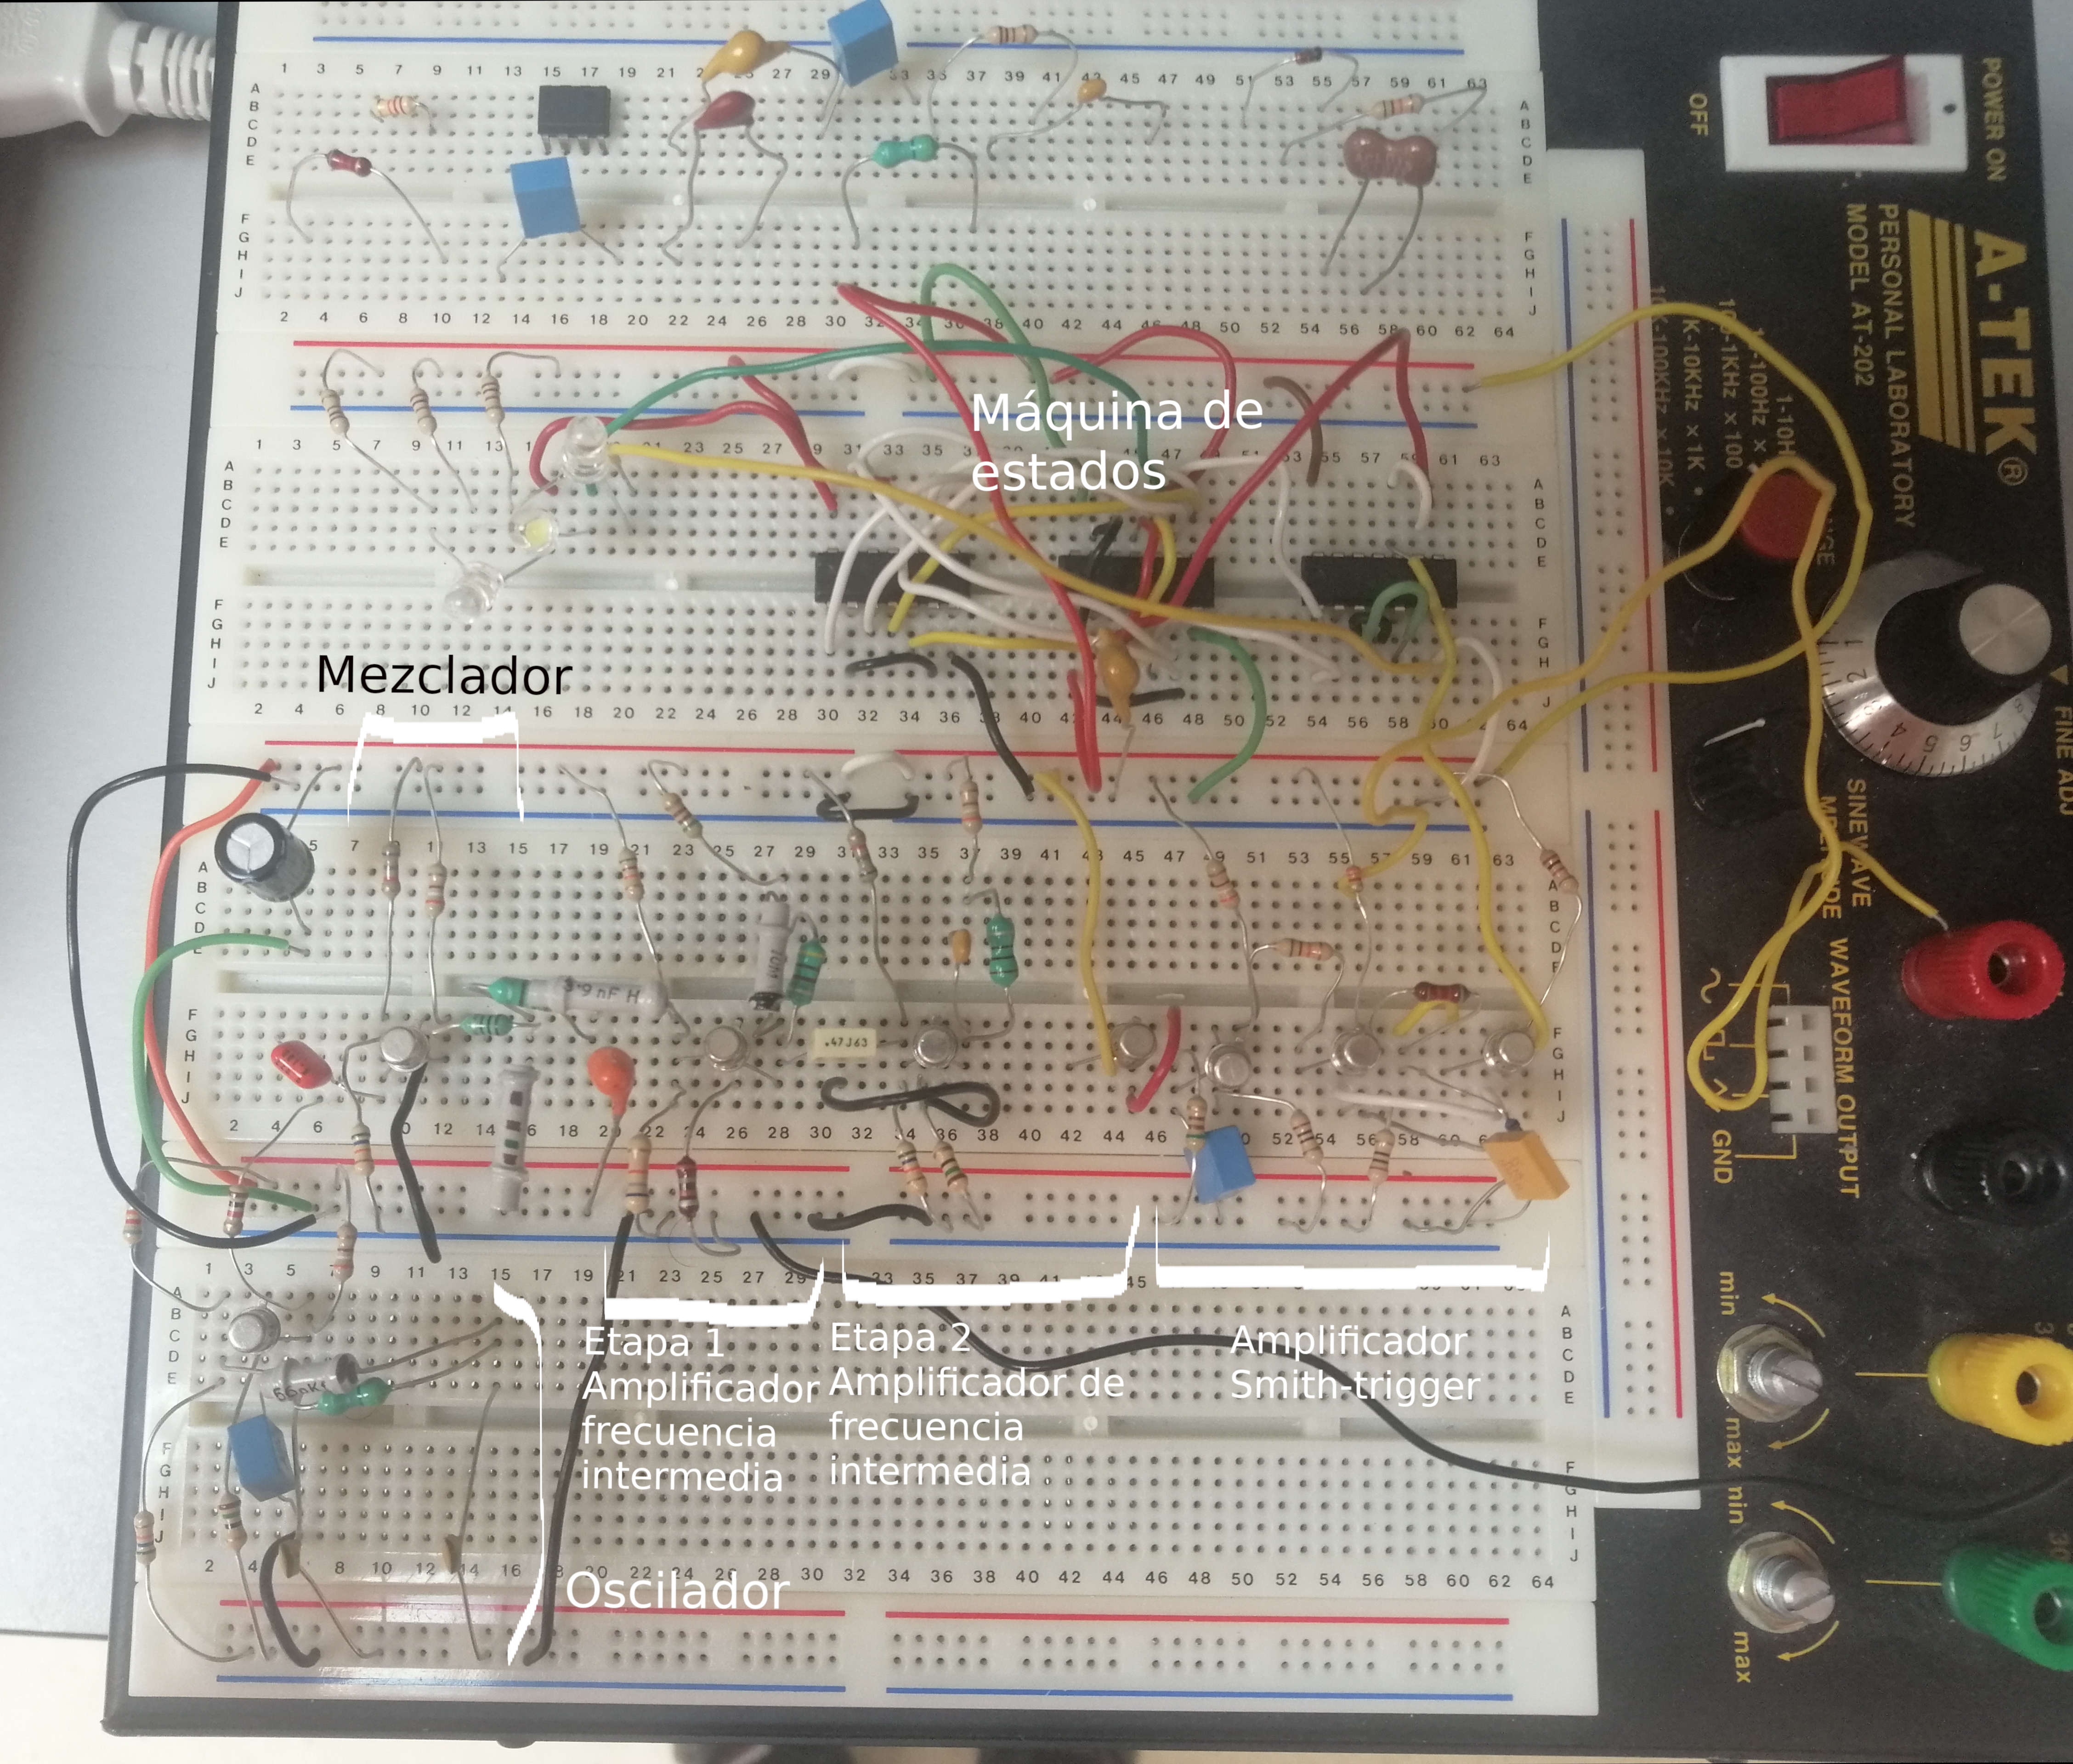
\includegraphics[scale=.7, width=.7\textwidth]{crono_general2}
    \caption{Implementaci\'on del receptor superheterodino de FM completo}
    \label{fig:crono_general}
\end{figure}

\paragraph{Motivos de reemplazo}
El diseño del circuito digital era correcto. Sin embargo, al realizar la integración con el receptor daba muchos problemas debido a que la señal de output del receptor no era fiable. Esta señal, al no estar bien filtrada poseía componentes residuales de alta frecuencia que provocaban que el smith trigger metiera señales falsas. esto provocaba un comportamiento no deseado del circuito. 
\paragraph{}
Para solucionar este hecho, se hizo uso de un microcontrolador. El micro abre una inmensidad de posibilidades como la recepci\'on de múltiples canales, reprogramable en función del uso específico, todo contenido en un menor espacio e incluso con un precio más económico.
